\documentclass[11pt]{article}
\usepackage[a4paper,left=1.5cm,right=1.5cm,top=1.5cm,bottom=1.5cm]{geometry}
\usepackage{fancyhdr}
\renewcommand{\headrulewidth}{1pt}
\fancyhead[C]{\textbf{[LINMA1170] Solveurs directs}}
\fancyhead[L]{Décembre 2018}
\fancyhead[R]{Gilles Peiffer [24321600]}

\usepackage[T1]{fontenc}
\usepackage[utf8]{inputenc}
\usepackage[french]{babel}
\usepackage{graphicx}
\usepackage{subcaption}
\usepackage{csquotes}
\usepackage{mathtools,amssymb}
\usepackage[binary-units=true,separate-uncertainty = true,multi-part-units=single]{siunitx}
\usepackage{float}
\usepackage[linktoc=all]{hyperref}
\hypersetup{breaklinks=true}
\setlength{\parskip}{1ex plus 0.5ex minus 0.2ex}
\newcommand{\hsp}{\hspace{20pt}}
\newcommand{\HRule}{\rule{\linewidth}{0.5mm}}
\graphicspath{{img/}}
\usepackage{caption}
\usepackage{textcomp}
\usepackage{array}
\usepackage{color}
\usepackage{tabularx,booktabs}
\usepackage{titlesec}
\usepackage{wrapfig}
\titlespacing{\section}{0pt}{\parskip}{-\parskip}
\titlespacing{\subsection}{0pt}{\parskip}{-\parskip}
\titlespacing{\subsubsection}{0pt}{\parskip}{-\parskip}
\pagestyle{fancy}
\DeclarePairedDelimiterX{\norm}[1]{\lVert}{\rVert}{#1}
\usepackage{listings}
\lstset{
	language=Python,
	numbers=left,
	numberstyle=\tiny\color{gray},
	basicstyle=\rm\small\ttfamily,
	keywordstyle=\bfseries\color{dkred},
	frame=single,
	commentstyle=\color{gray}=small,
	stringstyle=\color{dkgreen},
	%backgroundcolor=\color{gray!10},
	%tabsize=8, % Thank you Papa Torvalds
	%rulecolor=\color{black!30},
	%title=\lstname,
	breaklines=true,
	framextopmargin=2pt,
	framexbottommargin=2pt,
	extendedchars=true,
	inputencoding=utf8,
}
\DeclareMathOperator{\dens}{\mathrm{dens}}

\begin{document}
\section*{Introduction}
Pour ce devoir, il était demandé d'écrire des fonctions en langage Python permettant de résoudre éfficacement un système d'équations linéaires issu d'un modèle d'éléments finis appelé \lstinline[language=bash]{ccore}.
Le devoir se divise en deux tâches: d'abord la résolution d'un système en format plein et puis en format creux.

\section{Format plein}
\label{sec:dense}
Dans la partie en format plein du devoir, le but était d'étudier la densité de la factorisation \textsc{lu} en place d'une matrice $A \in \mathbb{C}^{n \times n}$ de faible densité.
Pour faire cela, il a fallu écrire une fonction capable de faire cette factorisation: \lstinline|LUfactorize|.
Elle prend en argument la matrice $A$ et décompose celle-ci en un produit d'une matrice triangulaire supérieure $U$ et d'une matrice triangulaire inférieure à diagonale unité $L$ de sorte à ce que $A = LU$.

Pour résoudre le système, il suffit alors de d'abord calculer $Ly = b$ par substitution avant pour trouver $y$, puis de résoudre $Ux = y$ par substitution arrière pour trouver $x$.
\lstinline|LUsolve| résout ainsi le système $Ax = b$.
\subsection{Étude de la densité de la décomposition \textsc{lu}}
\label{sec:fulldens}
Comme la matrice $A$ est issue d'un modèle d'éléments finis, elle contient beaucoup d'entrées nulles.
La densité d'une matrice est définie comme $ \dens A  = \frac{\textnormal{nnz}}{n^2}$, où $\textnormal{nnz}$ est défini comme le nombre d'éléments non nuls de $A$. On note la densité de $A$ après factorisation en place comme $\dens(LU)$ par simplicité.

Afin de faire une étude correcte de l'évolution de la densité de la matrice $A$ après sa décomposition \textsc{lu} en place, plusieurs graphes ont été réalisés.
Ils sont représentés à la Figure~\ref{fig:full_density}.
\begin{figure}[H]
	\centering
	\begin{subfigure}[t]{0.27\textwidth}
		\centering
		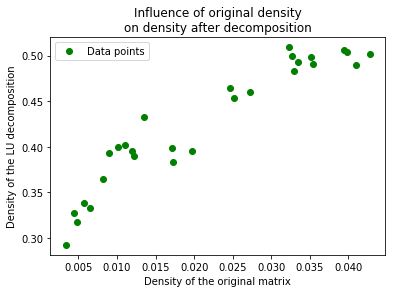
\includegraphics[width=\linewidth]{dens_adens_lu.png}
		\caption{Valeur de $\dens(LU)$ en fonction de $\dens A$.}
		\label{fig:a_dens__lu_dens}
	\end{subfigure}\hfill
	\begin{subfigure}[t]{0.27\textwidth}
		\centering
		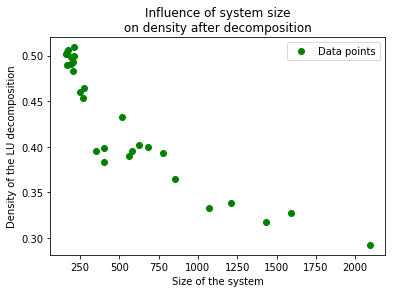
\includegraphics[width=\linewidth]{dens_lu__size.png}
		\caption{Influence de la taille du système sur $\dens (LU)$.}
		\label{fig:dens_lu__size}
	\end{subfigure}\hfill
	\begin{subfigure}[t]{0.27\textwidth}
		\centering
		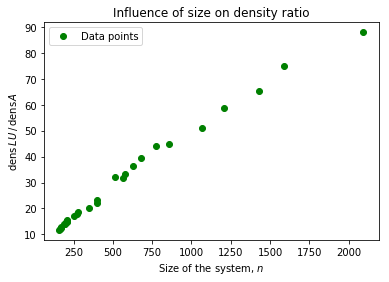
\includegraphics[width=\linewidth]{dens_ratio.png}
		\caption{Rapport entre $\dens(LU)$ et $\dens A$ en fonction de $n$.}
		\label{fig:dens_ratio}
	\end{subfigure}
	\caption{Différents graphes pertinents pour l'analyse de densité en section~\ref{sec:fulldens}.}
	\label{fig:full_density}
\end{figure}
On remarque que plus la matrice devient grande, plus elle devient creuse; c'est une propriété du modèle d'éléments finis. Sur le graphe de la Figure~\ref{fig:a_dens__lu_dens}, on remarque que la densité de la factorisation augmente lorsque la densité de $A$ augmente. Cependant, comme expliqué à la section~\ref{sec:rcmk}, ce rapport n'est que qualitatif et dépend du contenu de la matrice $A$.

En combinant le fait que la densité de $A$ diminue plus le système devient grand, et que la densité de la factorisation diminue lorsque la densité de $A$ devient plus petite, on peut prédire par transitivité que plus le système devient grand, plus la densité de sa factorisation \textsc{lu} va diminuer.
C'est ce qu'on observe sur le graphe de la Figure~\ref{fig:dens_lu__size}.
Finalement, le rapport de la densité de la matrice après factorisation sur sa densité avant factorisation est représenté comme une fonction de la taille du système à la Figure~\ref{fig:dens_ratio}.

\subsection{Complexité temporelle de \texttt{LUsolve}}
Le solveur \lstinline|LUsolve| fait deux choses séquentiellement, et la complexité totale est donc la somme des deux complexités partielles.
\subsubsection{Complexité temporelle de \texttt{LUfactorize}}
Il s'agit ici de calculer le nombre d'opérations pour une décomposition \textsc{lu} en place. Pour cela, on se réfère au livre de référence\footnote{Trefethen, Lloyd N. \& Bau, David \textrm{III}. (1997). \textit{Numerical Linear Algebra}. Philadelphia: PA, SIAM.} pp. 151--152.
Le nombre d'opérations de l'Algorithme~20.1 est dominé par l'opération vectorielle $u_{j, k:n} = u_{j, k:n} - \ell_{jk} u_{k, k:n}$.
Soit $l = n - k + 1$ la longueur des vecteurs lignes étant manipulés.
On voit que l'opération dominante effectue une multiplication scalaire-vecteur et une soustraction entre vecteurs. Le nombre de \emph{flops} est alors de $2l$.
Pour chaque valeur de $k$, l'indice de la boucle extérieure, la boucle intérieure est répétée pour toutes les lignes de $k+1$ jusque $n$.
La complexité de \lstinline|LUfactorize|, $d(n)$, est donc
\[
d(n) \sim \sum_{k=1}^{n} \underbrace{(n - k)}_{j} 2(n - k + 1) = 2 \sum_{j=0}^{n-1} j (j+1) = 2 \sum_{j=0}^{n-1} j^2  + 2 \sum_{j=0}^{n-1} j = 2 \left(\frac{n^3}{3} - \frac{n^2}{2} + \frac{n}{6}\right) + 2 \left(\frac{n^2}{2} - \frac{n}{2}\right) \sim \frac{2 n^3}{3}\,. 
\]
\subsubsection{Complexité temporelle des substitutions}
On sait que la substitution arrière effectue $\frac{n^2 - n}{2}$ soustractions, $\frac{n^2 - n}{2}$ multiplications et $n$ divisions.
Pour la substitution avant, les opérations effectuées sont $\frac{n^2 - n}{2}$ soustractions et $\frac{n^2 - n}{2}$ multiplications.
Pour obtenir ces résultats, calculons la complexité temporelle des substitutions, $\aleph(n)$, qui est alors la somme des complexités de chacune, c'est-à-dire
\[
\aleph(n) \sim \underbrace{\sum_{k=1}^{n} 2(\overbrace{n-k}^{j})}_{\textnormal{avant}} + \underbrace{\sum_{k=1}^{n} \big(2(n - k) + 1 \big)}_{\textnormal{arrière}} \sim 2 \sum_{j=0}^{n-1} j + 2 \sum_{j=0}^{n-1} j + n = 4 \left(\frac{n^2}{2} - \frac{n}{2}\right) + n \sim 2 n^2\,.
\]
\subsubsection{Complexité totale}
\begin{wrapfigure}{r}{6cm}
	\centering
	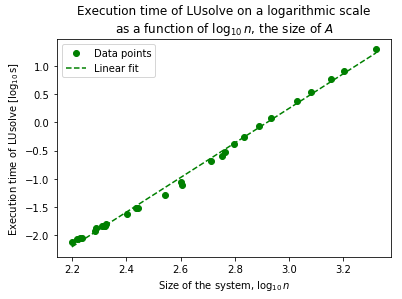
\includegraphics[width=0.32\textwidth]{lusolve_time.png}
	\caption{Temps d'exécution de \lstinline|LUsolve| en fonction de $n$. La pente de $3$ montre la relation cubique.}
	\label{fig:lusolve_time}
\end{wrapfigure}
Comme dit plus haut, pour trouver $s(n)$, la complexité temporelle totale, il suffit de sommer les deux complexités (comme les opérations se font en série).
On trouve alors
\[
s(n) = d(n) + \aleph(n) \sim \frac{2n^3}{3} + 2n^2 \sim \frac{2n^3}{3}\,.
\]
Comme on peut le voir, l'étape de factorisation est dominante pour la complexité temporelle. On voit sur le graphe de la Figure~\ref{fig:lusolve_time} que cette prédiction théorique est confirmée expérimentalement. Mentionnons finalement que comme les matrices sont issues d'un modèle d'éléments finis, elles sont symétriques (hermitiennes) et définies positives; il n'est alors pas nécessaire de rajouter une vérification pour éviter les divisions par zéro dans \lstinline|LUfactorize|. Ceci se démontre par le critère de Sylvester.
\section{Format creux}
Les matrices issues de \lstinline[language=bash]|ccore| sont très creuses.
Il serait donc intéressant de trouver une manière de résoudre le système sans avoir à faire autant de calculs.
Pour faire cela, nous utilisons le format \textsc{csr} et la fonction \lstinline|CSRformat| afin avoir une représentation de la matrice qui n'utilise pas autant de mémoire.
Une fois celle-ci obtenue, il est possible d'améliorer la complexité de la résolution du système par factorisation \textsc{lu}.
\subsection{Performances de \texttt{CSRformat}}
\label{sec:csrformat}
\begin{wrapfigure}{r}{6cm}
	\centering
	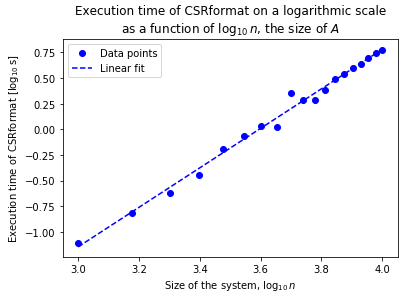
\includegraphics[width=0.32\textwidth]{csrformat.png}
	\caption{Temps d'exécution de \lstinline|CSRformat| en fonction de $n$. La pente de $2$ montre la relation quadratique.}
	\label{fig:csrformat}
\end{wrapfigure}
La fonction \lstinline|CSRformat| parcourt toute la matrice, ligne par ligne, en copiant toutes les entrées non nulles dans un vecteur \lstinline|sA|, leurs indices de colonne dans \lstinline|jA| et l'indice de leur premier élément non nul dans \lstinline|iA|.
On voit donc facilement que cette fonction doit avoir une complexité temporelle de $\Theta(n^2)$. Les opérations les plus coûteuses effectuées sont le parcours de la matrice pour trouver la valeur de $\textnormal{nnz}$ en $\Theta(n^2)$ et la recherches d'indices et de valeurs d'éléments non nuls sur une ligne, en $\Theta(n^2)$ au total pour $n$ lignes.
La complexité totale est donc également en $\Theta(n^2)$, ce qui se voit sur le graphe de la Figure~\ref{fig:csrformat}.
\subsection{Complexité temporelle de \texttt{LUcsrsolve}}
\label{sec:LUcsrsolve}
La fonction \lstinline|LUcsrsolve| est une version optimisée de \lstinline|LUsolve| spécifiquement pour les matrices creuses.
Il est important pour les solveurs creux de connaître la bande de la matrice $A$.
Définissons la largeur de bande $k$ de $A$ comme étant
\[
k = \max(k_1, k_2)\,, \quad \textnormal{où} \quad a_{ij} = 0 \quad \textnormal{si} \quad j < i - k_1 \quad \textnormal{ou} \quad j > i + k_2\,; \quad k_1, k_2 \ge 0\,.
\]
En effet, une des propriétés de la factorisation \textsc{lu} est que lors de la décomposition, des nouvelles entrées non nulles peuvent apparaître mais uniquement à l'intérieur de la bande de la matrice (phénomène de \emph{fill-in}). On peut donc préallouer facilement cette bande, la remplir au fur et à mesure de la factorisation, et n'avoir qu'à considérer une partie de cette bande (et donc de la matrice $A$) lors des substitutions. Pour calculer la complexité de la fonction \lstinline|LUcsrsolve|, il faut observer qu'elle sera égale à la somme des complexités de \lstinline|LUcsr| et de deux substitutions modifiées.
\subsubsection{Complexité temporelle de \texttt{LUcsr}}
La fonction \lstinline|LUcsr| a une complexité qui dépend de plusieurs étapes: d'abord le calcul de la largeur de bande en $\Theta(n)$ grâce au format \textsc{csr} en utilisant le vecteur \lstinline|iA|; ensuite, la préallocation de vecteurs de taille au plus $nk$ en $\mathcal{O}(nk)$ et finalement la réelle décomposition \textsc{lu} creuse en $\lambda(n, k)$. Pour trouver $\lambda(n, k)$, on observe que la boucle intérieure fait deux opérations: (une multiplication et une soustraction), et on calcule (en idéalisant un peu)
\[
\lambda(n, k) \in \mathcal{O}\Bigg(\sum_{i=0}^{n-1}\ \  \sum_{j = i+1}^{\min(i+k_1+1, n)-1} \ \ \sum_{m = i+1}^{\min(i+k_2+1, n)-1} 2\Bigg) \subseteq \mathcal{O}\Bigg(2 \sum_{i=0}^{n-1} k_1 k_2\Bigg) \subseteq \mathcal{O}(2nk_1k_2) \subseteq \mathcal{O}(n k^2)\,.
\]
\subsubsection{Complexité des substitutions modifiées}
Dans les substitutions modifiées, on peut utiliser le fait que seule la partie non nulle de la matrice nous intéresse. On écrit alors la complexité $\sigma(n, k)$ des deux substitutions en série comme
\[
\sigma(n, k) \sim \underbrace{\sum_{i=0}^{n} \ \ \sum_{j=\max(0, i-k_1+1)}^{i-1} 1}_{\textnormal{avant}} + \underbrace{\sum_{i=0}^{n} \ \ \sum_{j=i+1}^{\min(i+k, n)-1} 1}_{\textnormal{arrière}} \sim nk_1 + nk_2 \sim 2nk \in \mathcal{O}(nk)\,.
\]
\subsubsection{Complexité totale de \texttt{LUcsrsolve}}
Comme dit plus haut, ces opérations se font toutes en série, et la complexité totale $t(n, k)$ s'écrit alors
\[
t(n, k) \in \mathcal{O}(nk^2 + nk) \subseteq \mathcal{O}(nk^2)\,.
\]
La factorisation est donc l'étape contribuant le plus à la complexité temporelle.
\subsection{Numérotation \foreignquote{french}{reverse Cuthill-McKee}}
\label{sec:rcmk}
Comme expliqué à la section~\ref{sec:LUcsrsolve}, la complexité de la fonction \lstinline|LUcsrsolve| dépend du carré de la largeur de bande.
Il serait donc intéressant d'utiliser un algorithme de renumérotation des n\oe{}uds tel que \textsc{rcmk} pour diminuer cette largeur de bande. Cet algorithme n'influence pas uniquement la complexité en temps mais aussi en mémoire: lors du \emph{fill-in} de la décomposition \textsc{lu}, plus la bande est petite, plus on peut borner la densité de la matrice résultant de la factorisation en place.
\begin{figure}[H]
	\centering
	\begin{subfigure}[t]{0.27\textwidth}
		\centering
		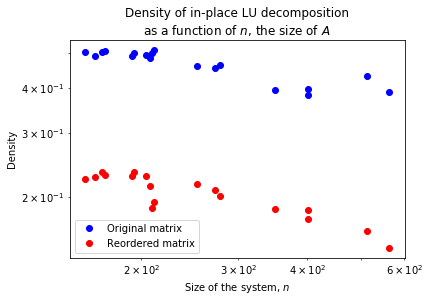
\includegraphics[width=\linewidth]{rcmk_dens.png}
		\caption{Comparaison entre la densité de la factorisation avec et sans \textsc{rcmk}.}
		\label{fig:rcmk_dens}
	\end{subfigure}\hfill
	\begin{subfigure}[t]{0.27\textwidth}
		\centering
		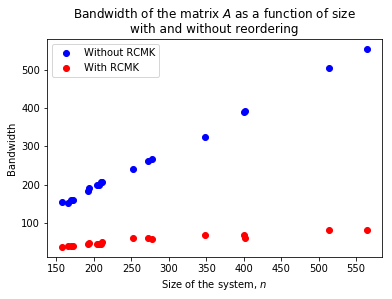
\includegraphics[width=\linewidth]{bandwidth.png}
		\caption{Influence de \textsc{rcmk} sur la largeur de bande de $A$.}
		\label{fig:bandwidth}
	\end{subfigure}\hfill
	\begin{subfigure}[t]{0.2\textwidth}
		\centering
		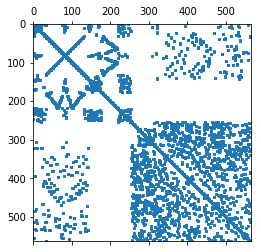
\includegraphics[width=\linewidth]{spy.png}
		\caption{Matrice $A$ sans renumérotation \textsc{rcmk}.}
		\label{fig:spy}
	\end{subfigure}\hfill
	\begin{subfigure}[t]{0.2\textwidth}
		\centering
		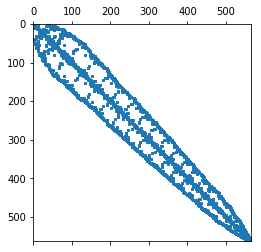
\includegraphics[width=\linewidth]{spy_rcmk.png}
		\caption{Matrice $A$ avec renumérotation \textsc{rcmk}.}
		\label{fig:spy_rcmk}
	\end{subfigure}
	\caption{Influence de la renumérotation \textsc{rcmk} sur la densité de $A$.}
	\label{fig:rcmk}
\end{figure}

Sur la Figure~\ref{fig:rcmk}, on peut voir que la densité de la factorisation \textsc{lu} diminue lorsque la matrice est permutée (Figure~\ref{fig:rcmk_dens}) et que la largeur de bande de la matrice $A$ diminue (et augmente beaucoup moins rapidement) lorsque la matrice est permutée (Figure~\ref{fig:bandwidth}).
Les Figures~\ref{fig:spy}~et~\ref{fig:spy_rcmk} donnent une vue qualitative.


\subsection{Complexité de \texttt{LUcsrsolve} avec renumérotation \textsc{rcmk}}
Afin d'évaluer l'utilité de cette renumérotation, il est intéressant de regarder l'évolution de la complexité lorsqu'on applique la permutation. Il faut alors rajouter deux étapes à la fonction: le calcul de la permutation optimale (fonction \lstinline|RCMK|) et son application.
\subsubsection{Complexité du calcul de la permutation}
\begin{wrapfigure}{R}{6cm}
	\centering
	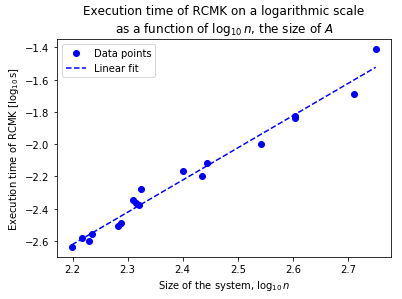
\includegraphics[width=\linewidth]{rcmk_exec.png}
	\caption{Temps d'exécution pour le calcul de la permutation \textsc{rcmk}.}
	\label{fig:rcmk_exec}
\end{wrapfigure}
Soit $M \in \{0, 1\}^{n \times n}$ la matrice telle que $m_{ij} = 1$ si $a_{ij} \ne 0$ et $0$ sinon, et soit $G(E, V)$ le graphe dont $M$ est la matrice d'adjacence, avec $E$ l'ensemble des arêtes et $V$ l'ensemble des n\oe{}uds.
L'étape dominante pour la complexité temporelle est le fait de devoir trier à chaque itération la liste des n\oe{}ds adjacents au n\oe{}ud venant de sortir de la file.
Or nous pouvons borner la taille de cette liste de n\oe{}uds adjacents par le degré maximal dans le graphe $G$, $\Delta(G)$.
On remarque alors que pour toute permutation de la matrice (toute renumérotation des n\oe{}uds), et donc en particulier pour la permutation \textsc{rcmk}, le degré maximal est inférieur au double de la largeur de bande augmenté de $1$ (pour compter l'élément diagonal): $\Delta(G) \le k_1 + k_2 + 1 \le 2k + 1$.
En supposant qu'un algorithme de tri avec une complexité dans le pire cas linéarithmique, tel que \emph{mergesort}, soit utilisé, on peut alors dire que la fonction \lstinline|RCMK| a une complexité $r(G)$ en $\mathcal{O}\big(|V| \Delta \log \Delta \big)$, ou bien, avec les paramètres de notre système \textsc{rcmk}, $n$ et $k$, 
\[
r(n, k) \in \mathcal{O}\big(n (2k+1) \log(2k+1)\big) \subseteq \mathcal{O}(nk \log k)\,.
\]
Le temps d'exécution de la fonction \lstinline|RCMK| est montré sur la Figure~\ref{fig:rcmk_exec}.
\subsubsection{Complexité de l'application de la permutation}
Pour permuter la matrice, on peut imaginer qu'il faut permuter d'abord les lignes puis les colonnes. Pour les lignes, il faut donc déplacer au plus $2nk$ éléments (comme chacune des $n$ lignes a au plus de l'ordre de $2k$ entrées), et pour les colonnes la même chose.
Il est alors possible d'appliquer la permutation en $\mathcal{O}(nk)$.
\subsubsection{Complexité de \texttt{LUcsrsolve} avec renumérotation \textsc{rcmk}}
La complexité totale $\tau(n, k)$ pour \lstinline|LUcsrsolve| avec renumération est alors (en comptant toujours la complexité de \lstinline|LUcsr|)
\[
\tau(n, k) \in \mathcal{O}(nk^2 + nk \log k + nk) \subseteq \mathcal{O}(nk^2)\,,\quad \textnormal{car} \quad \lim_{(n, k) \to (+\infty, +\infty)} (nk^2 + nk \log k) = \lim_{(n, k) \to (+\infty, +\infty)} nk^2\,.
\]
\begin{wrapfigure}{R}{6cm}
	\centering
	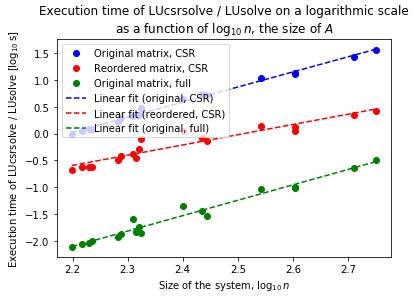
\includegraphics[width=\linewidth]{all_exec_time.png}
	\caption{Temps d'exécution pour les différents solveurs.}
	\label{fig:all_exec_time}
\end{wrapfigure}
C'est la même complexité que pour \lstinline|LUcsrsolve| sans renumérotation, mais on remarque que comme la largeur de bande a fortement diminué, la résolution du système sera beaucoup plus rapide pour les matrices creuses.
C'est aussi ce qu'on observe sur la Figure~\ref{fig:all_exec_time}.
On remarque que le solveur plein est plus rapide pour les matrices de ces tailles (grâce à la vectorisation et aux routines optimisées de \lstinline[language=bash]|BLAS|), mais la pente pour le solveur avec \textsc{rcmk} est plus petite, et à partir d'un certain $n_0 \gg 0$, la résolution avec permutation sera plus rapide.

Un autre point intéressant est que dans le cas de matrices très mal numérotées ($k \approx n$), l'algorithme creux devient un simple algorithme de factorisation en $\mathcal{O}(n^3)$ et sa pente est égale à la pente pour le solveur plein.

\section*{Conclusion}
La résolution de systèmes algébriques est un aspect important de l'analyse numérique, et la décomposition \textsc{lu} est souvent le meilleur choix pour le faire rapidement. Malgré la simplicité de l'algorithme, il permet de résoudre rapidement des systèmes de grande taille.
Pour les matrices issues d'un modèle d'éléments finis, on sait qu'elles sont creuses et hermitiennes. Il est alors possible de les réordonner par une algorithme tel que \textsc{rcmk} afin de diminuer le temps pour résoudre le système en profitant de l'aspect \foreignquote{french}{bande} de telles matrices.
\end{document}